\documentclass{beamer}
\usetheme{Warsaw}
%\usecolortheme{seahorse}
\usepackage{graphicx}
\usepackage[utf8]{inputenc}
\usepackage[T1]{fontenc}
\title{C++0x performance improvements}
\author{Łukasz Milewski}
\institute{Uniwersytet Wrocławski}
\date{\today, Wrocław}

\begin{document}

\begin{frame}
  \titlepage
\end{frame}

\begin{frame}
  \tableofcontents
\end{frame}

\section{move semantics and perfect forwarding}
\begin{frame}{rationale}
  \begin{block}{Why?}
    \begin{itemize}
    \item Eliminate expensive copying
    \item Solve problems with generic forwarding
    \item Solve usability problems where binding a rvalue to non-const reference is not a logical error
    \end{itemize}
  \end{block}
\end{frame}

\subsection{lvalue, rvalue and rvalue reference}
\begin{frame}{expression category taxonomy}
  \begin{center}
    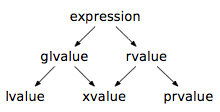
\includegraphics[5cm]{valuetaxonomy.png}
  \end{center}
\end{frame}

\begin{frame}{lvalue, rvalue, rvalue reference}
  \begin{block}{lvalue}
    \begin{itemize}
    \item Can appear on left-hand side of an assignment expression
    \item if E is expr of pointer type, then *E is an lvalue
    \item calling function whose return type is an lvalue reference is lvalue
    \end{itemize}
  \end{block}

  \begin{block}{rvalue}
    \begin{itemize}
    \item can appear on right-hand side of an assignment expression
    \item xvalue
    \item temporary object
    \item value that is not assosiated with an object
    \end{itemize}
  \end{block}
\end{frame}

\begin{frame}{example}
  see rvalue\_lvalue.cpp
\end{frame}

\begin{frame}
  \begin{block}{rvalue reference}
    \begin{itemize}
    \item T& - lvalue reference
    \item T&& - rvalue reference
    \item const T&&
    \item binds to lvalues and rvalues
    \item binds to rvalue even if not const qualified
    \end{itemize}
  \end{block}
\end{frame}

\begin{frame}{binding}
  \begin{block}{binding}
  \item lvalue ref binds to lvalue
  \item const lvalue ref binds to everything
  \item rvalue ref binds to lvalue and nonconst rvalue
  \item const rvalue ref binds to everything
  \end{block}
  see binding.cpp
\end{frame}

\begin{frame}{overload resolution}
  rvalue\_ref\_resolution.cpp
\end{frame}

\subsection{performance improvements}
\begin{frame}{std::vector::emplace\_back}
  \begin{block}{move object when vector grows}
    \begin{itemize}
    \item c++03 copies all objects in vector to new memory
    \item why do that if these objects are about to be destroyed?
    \item c++0x moves all objects in vector to new memory
    \end{itemize}
  \end{block}
\end{frame}

\begin{frame}{string concatanation}
  std::string tmp = std::string("ala") + " " + "ma" + " " + "kota" + "!";
  \begin{block}{c++03}
    \begin{itemize}
    \item every call to operator+ returns a temporary object
    \item a lot of copying
    \item a lot of dynamic memory allocation
    \item no COW
    \item small strings optimization applies only for small strings
    \end{itemize}
  \end{block}

  \begin{block}{c++0x}
    \begin{itemize}
    \item every call to operator+ returns a temporary object
    \item second temporary string is constructed by stealing the memory owned by the first one
    \end{itemize}
  \end{block}
\end{frame}

\begin{frame}{RVO & NRVO vs move}
  see rvo.cpp
\end{frame}

\subsection{usability improvements}


\section{constexpr}
\section{POD modifications}
\section{multithreading}
\section{alignment}
\section{unique\_ptr}

\end{document}
